% ----------------------------------------------------------
% Arquivo contendo a introdução do trabalho sobre algoritmo genético
%
% ----------------------------------------------------------
\chapter{Introdução}
% ----------------------------------------------------------

\section{Algoritmos evolucionários}

Os algoritmos evolucionários são um subconjunto da computação evolutiva, sendo essa um conjunto de algoritmos para busca de soluções ótimas globais. A computação evolutiva é baseada na evolução das espécies definida na biologia, e assim os algoritmos evolucionários se baseiam em processos encontrados na natureza de seleção, reprodução e mutação das espécies, com o propósito de otimizar a solução para um problema definido.

Um problema de otimização é definido como maximizar, ou minimizar, $f(x)$ sujeito a \(g_i(x) \leq 0\,i = \{1,\ldots, m\}\), e \(h_j(x) = 0, j=\{1,\ldots,n\}\) com \(x \in \Omega \). A solução maximiza, ou minimiza, o escalar \(f(x)\) onde \(x\) é um vetor com dimensão \(n\), \(x=\{x_1,x_2,\ldots,x_n\}\) do espaço de soluções \(\Omega\). \cite{Coello2007} 

Dessa forma o problema de otimização tem os seguintes componentes:
\begin{itemize}
	\item Função objetivo \(f(x)\): função de avaliação que deve se minimizada ou maximizada;
	\item As restrições \(g_i(x)\) e \(h_j(x)\): definem limites para as soluções que são permitidas;
	\item Espaço de soluções \(\Omega\) :
		Conjunto com todas as possíveis soluções para o problema; 
\end{itemize}

De forma mais simplificada podemos escrever o problema de otimização como, sendo \(\Omega\) o espaço de soluções e a função \[ g: \Omega \to \mathbbm{R}\] e a solução o vetor \(x \in \Omega\) tal que \[ \arg \min \limits_{x \in \Omega} g(x)\] que pode facilmente ser convertido para um problema de maximização usando \(-g(x)\)

Para atingir esse objetivo os algoritmos evolutivos trabalham com uma população de indivíduos que indicaremos como soluções candidatas para o problema. Baseado na avaliação de cada individuo com relação ao seu ambiente, em nosso contexto a função de avaliação, e usando operadores definidos para seleção e evolução, a população vai sendo modificada até que se atinja um resultado satisfatório para o problema. Assim como no processo de evolução das espécies definidos por Darwin, que introduziu o conceito de seleção natural  através da sobrevivência do mais apto, os indivíduos da população que tem melhores avaliações, ou seja, que melhor se adaptam ao ambiente, possuem mais probabilidade de sobrevivência e assim se reproduzirem. 

Existem vários métodos para se otimizar um problema conforme pode ser visto na \autoref{fig:classificacao_metodos_busca}. Existem os métodos enumerativos, que se tornam impraticáveis quando o \(\Omega\) é muito grande, pois o algoritmo deveria testar todas as soluções possíveis. Os algoritmos determinísticos são os mais eficientes em determinadas condições, como por exemplo o comportamento de \(f(x)\). Se a função objetivo possui múltiplos máximos (ou mínimos) alguns algoritmos determinísticos, como o \textit{hill-climbing} por exemplo, podem ficar 'presos' em soluções locais e não encontrar a solução global. A última categoria, onde se encontram também os algoritmos evolucionários, são os estocásticos (ou randômicos). Possuem a vantagem de não ficar presos em soluções locais, porém nem sempre obterão a melhor solução.

\begin{figure}
	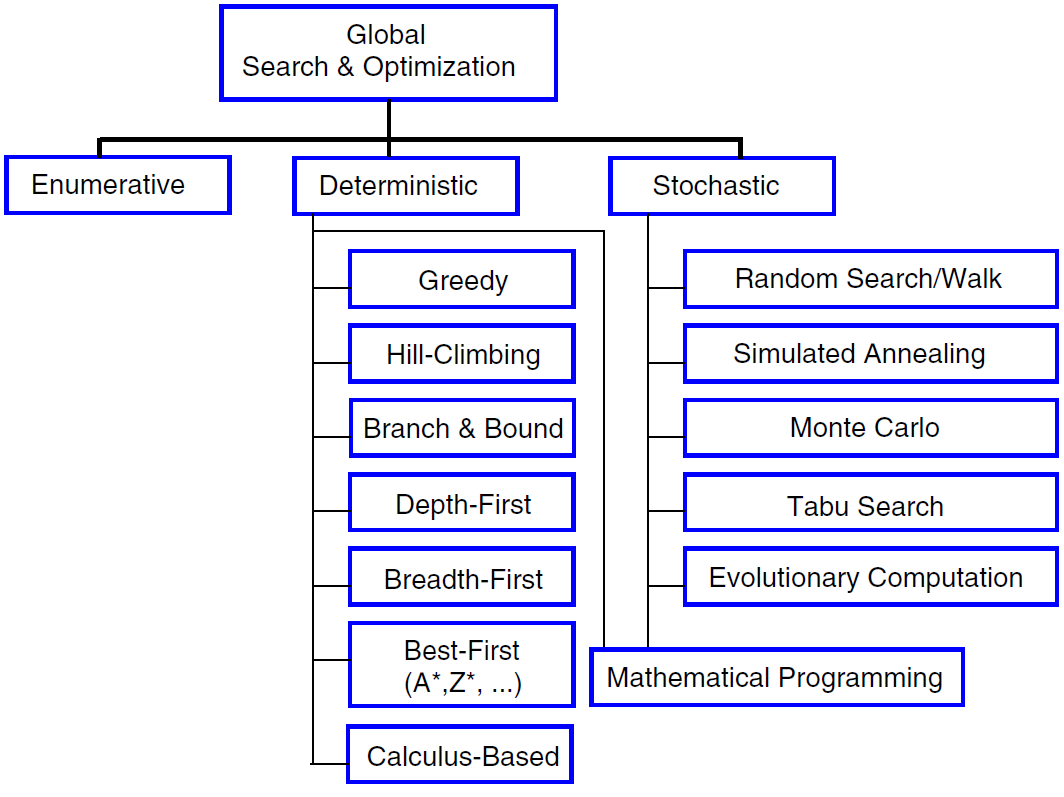
\includegraphics[width=\linewidth]{imagens/classificacao_metodos_busca.png}
	\caption{Técnicas de otimização global - \cite{Coello2007}}
	\label{fig:classificacao_metodos_busca}
\end{figure}

Dentre a categoria dos métodos estocásticos existem os que são completamente aleatórios, como a busca randômica (ou passeio aleatório), e os que são de alguma forma guiado como o método de Monte Carlo por exemplo. O algoritmo evolucionário se encaixa nessa ultima definição, onde existem componentes aleatórios atuando na seleção e reprodução dos indivíduos mas de forma guiada pelos resultados da função de avaliação.

De acordo com \citeauthor{Linden2008}, os AE são \textbf{heurísticas}\footnote{Heurísticas são algoritmos polinomiais que usualmente tendem a encontrar soluções ótimas ou próximas delas, mas sem garantias} que não asseguram obter o melhor resultado possível, e além disso o resultado pode diferir entre as execuções do algoritmo.

Para \citeauthor{Sivanandam2007}, um algoritmo evolucionário são processos estocásticos e iterativos que operam em um conjunto de indivíduos (população). Cada individuo representa uma possível solução para o problema de otimização ou busca, sendo que os parâmetros estão de alguma forma codificados nesses indivíduos. A população inicial é gerada aleatoriamente e são avaliados usando alguma função, que determina o quão bem o indivíduo responde ao problema. Esse valor determina a direção de busca do algoritmo. 

\section{Biologia}
A ideia por trás dos algoritmos evolucionários e por consequência do algoritmo genético, é a teoria de evolução das espécies na natureza de \textbf{Darwin}, onde a sobrevivência de cada indivíduo é determinada por como ele se adapta ao seu meio. Assim aqueles que conseguiam vantagens sobre os demais por ter uma maior sobrevivência se reproduziam mais, e assim, passavam para as próximas gerações essas características que os diferenciavam. Darwin chamou de seleção natural esse mecanismo da sobrevivência dos mais aptos.

Contudo Darwin não sabia explicar como essa informação era passada dos ancestrais para os descendente, onde então entram as descobertas de \textbf{Mendel}, que através dos conceitos de genética determinava como características eram compartilhadas entre pais e filhos. 

A unidade básica de informação é o gene, que é um bloco de sequências de DNA e o conjunto de genes formam o cromossomo. Cada gene tem um \textit{locus}, que define a região dentro do cromossomo onde está localizado, e possui um conjunto de valores possíveis chamados de alelos. Os genes controlam as características do indivíduo, sendo que a expressão dessas no individuo é denominada de fenótipo. Assim um conjunto específicos de genes define o genótipo do indivíduo que está associado a um fenótipo, que apresenta as características codificadas no genótipo e que podem ser modificadas pelo ambiente. 

Organismos com cromossomos combinados em pares são chamados de diplóides em contraste com os que não possuem pares, chamados de haplóides. Na natureza a maioria dos seres mais complexos que se reproduzem sexualmente são normalmente diplóides e possuem um ou mais pares de cromossomos sendo que sua quantidade e tamanho dependem de cada ser vivo.

Durante a reprodução ocorre a transmissão da informação que pode ser de dois tipos: assexuada e sexuada. Na reprodução assexuada, o organismo replica a si mesmo, presente mais em seres simples, não representa tanta diversidade pois como não existe combinação de material genético entre dois seres, ocorre apenas a retransmissão de material genético, somente sujeito a alterações por mutação na cópia.

Na reprodução sexuada de seres diplóides, há presença de dois indivíduos que compartilham seu material genético para formar um novo organismo. No inicio da reprodução, existe a cópia do material genético e recombinação, também chamado de \textit{crossover}(\autoref{fig:crossover_example}). Esse processo é feito com é feito com os cromossomos se cruzando, por isso o termo \textit{crossover},  um sobre o outro em um ou mais pontos havendo assim a troca nas sequências de genes. Após feita a recombinação, o material genético é divido em gametas que então são combinados com os gametas do outro pai para formar novamente um cromossomo diplódie completo, gerando assim os novos indivíduos. Para organismos haplóides é feita apenas a combinação das sequencias de cada pai.

\begin{figure}
	\begin{center}
	\includegraphics[width=0.5\textwidth]{imagens/cross_over.png}
	\caption{Exemplo de reprodução com crossover - \cite{Klug2011}}
	\label{fig:crossover_example}
	\end{center}
\end{figure}


Dentro da etapa de replicação do DNA podem ocorrer erros ou alterações influenciadas por fatores externos, gerando assim as mutações. Isso pode ser positivo, negativo ou não influenciar o resultado final, mas é um outro mecanismo que pode determinar a evolução das espécies.   

Combinando indivíduos que melhor se adaptaram as condições de sobrevivência, provavelmente deve gerar novos indivíduos que tenha características ainda melhores que seus antecessores. O outro caso pode acontecer também e o novo indivíduo ter piores condições de viver, e assim o processo de seleção natural levará esse espécime a extinção favorecendo outros que se sobressaíram na próxima geração.

A evolução então é um processo adaptativo onde através de mutações e recombinação entre os indivíduos, vão surgindo novas gerações que devem apresentar cada vez mais seres que se adaptam cada vez melhor ao ambiente.

\section{Algoritmo genético}

Alguns autores como \citeauthor{Mitchell1996}, \citeauthor{LeeJacobson2015}, \citeauthor{Kwong2001} entre outros citam eu o criador, ou quem primeiro especificou o algoritmo genético(\textit{Genethic Algorithm} ou GA) foi Holland em 1975 no livro \textit{"Adaptation in Natural and Artificial Systems"}. Nele Holland formaliza uma estrutura para sistemas adaptativos, e encaixa o GA como uma abstração para a evolução biológica.

Na estrutura criada por Holland para um problema bem posto de adaptação temos:
\begin{itemize}
	\item \( \mathscr{A} = \{ \mathcal{A}_1, \mathcal{A}_2, \ldots \} \) é um conjunto de estruturas do domínio.
	\item \( \Omega = \{ \omega_1, \omega_2, \ldots \} \) é um conjunto de operadores para modificar as estruturas de \( \mathscr{A} \).  Sendo \( \omega \in \Omega \) uma função \(\omega : \mathscr{A} \to \mathcal{P} \) onde \(\mathcal{P}\) é uma distribuição de probabilidades sobre \(\mathscr{A}\)
	\item \( \mathcal{I}\) é o conjunto de entradas do ambiente
	\item \( \tau : \mathcal{I} \times \mathscr{A} \to \Omega\) é o plano adaptativo baseado nas entradas e nas estruturas no intervalo de tempo \(t\) e determina os operadores a serem aplicados nesse intervalo.
\end{itemize}
Assim: 
\[\tau(\mathcal{I}(t), \mathscr{A}(t)) = \omega_t \in \Omega \text{ e } \omega(t)(\mathscr{A}(t)) = \mathcal{P}(t + 1)\]
onde \(\mathcal{P}(t + 1) \) é uma distribuição particular sobre \( \mathscr{A} \). \( \mathscr{A}(t+1) \) é determinado retirando uma amostra aleatória de \( \mathscr{A} \) de acordo com essa distribuição. \cite{Holland1992}

Ainda define os seguintes itens, \( \mathcal{T} \) como o conjunto de planos possíveis (\(\tau\)), \(\mathcal{E}\) como sendo o conjunto de ambientes possíveis e \(\mu_E(\mathscr{A}(t))\) como a função de avaliação com \( E \in \mathcal{E} \). 

Usando essa estrutura com a definição do algoritmo genético dado por Holland ....

